\documentclass[12pt]{exam}
\usepackage[spanish]{babel}
\usepackage{amsmath} % Para notación matemática
\usepackage{multicol} % Para crear columnas
\usepackage[left=10mm, right= 20mm, bottom= 20mm, top= 35mm, headsep=10mm, headheight=0mm]{geometry}
\usepackage{setspace}  
\usepackage{graphicx}
\renewcommand\partlabel{\thepartno)}
%%% DEFINICIONES PARA MODIFICAR APARIENCIA DEL ENCABEZADO%%%
\usepackage{etoolbox}
\makeatletter
\patchcmd{\@fullhead}{\hrule}{\hrule\vskip2pt\hrule height 2pt}{}{}
\patchcmd{\run@fullhead}{\hrule}{\hrule\vskip2pt\hrule height 2pt}{}{}
\makeatother
\pagestyle{headandfoot}
%\runningheadrule
\firstpageheadrule
\firstpageheader {\escuela \\ Curso: \curso}
                 {MATEMÁTICA \\ \tpnombre}
                  {\lugar \\ \today}  
%\runningheader{\includegraphics[width=0.1\textwidth]{logo.png}}
%{Matemática:Trabajo Práctico}
%{\today}
\firstpagefooter{Prof: \textit{Lucas H.Trejo}}{}{\thepage}
\runningfooter{Prof: \textit{Lucas H.Trejo}}{}{Pag. \thepage\ of \numpages}

%%%%%%%%%%%%%%%%%%%%%%%%%%%%%%%%%%%%%%%%%%%%%%%%%%%%%%%%%%%%%%%%%%%%%%%%%%%%%%%
                                       %%% REEMPLAZAR LOS PARÁMETROS AQUÍ    %%  
\newcommand{\escuela}{EES Nº 32}                                             %%             
\newcommand{\curso}{  5º 3ª}                                                  %%             
\newcommand{\tpnombre}{Funciones polinómicas}                     %%
\newcommand{\lugar}{La Plata}                                               %%
%%%%%%%%%%%%%%%%%%%%%%%%%%%%%%%%%%%%%%%%%%%%%%%%%%%%%%%%%%%%%%%%%%%%%%%%%%%%%%%


\begin{document}

 


\begin{questions}
    
    \question Escribir una función polinómica $f(x)$ cuyo gráfico sea el siguiente.
    \begin{figure}[h]
        \centering
        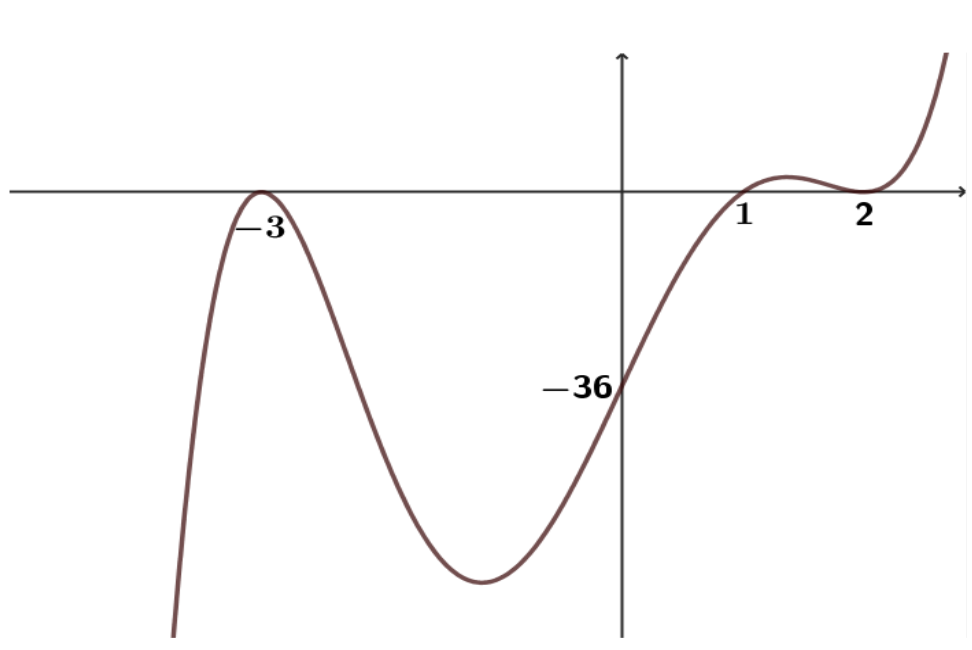
\includegraphics[width=.5 \linewidth]{hallar_fx.png}     
    \end{figure}
    
    \question Determinar una función polinómica y trazar un gráfico aproximado:

    \begin{parts}
        \part de grado 4 sabiendo que $C^0 = \{2; 4\}$, $C^- = \emptyset$ y $f(3) = \frac{1}{2}$.
        \part de grado 3 sabiendo que $C^- = (-\infty; -3) \cup (-3; 1)$ y la ordenada al origen es $y = -9$.
        \part de grado mínimo, cuya ordenada al origen sea $y = -10$, sus únicas raíces sean $-5$, $-1$, $3$ y $4$, y $C^+ = (-5; -1) \cup (4; +\infty)$.
    \end{parts}
     
\question La funcion $h(x) = 4x^3 - 6x^2 - 22x + 12 $ es el produto de $g(x)$ y $f(x)$.
 \begin{parts}    
 
\part ¿Puede ser que una de ellas sea $g(x) = -2x - 1$ ? Si les parece que sí encuentren $f$. Si les
parece que no, justificar.
\part ¿Y si fuera $g (x) = x - 1$?
\part Si es posible, escribir $ h(x) $ como produto de tres lineales. De no ser posible, explicar por
qué.
\end{parts}
    
    \question Dadas las funciones:\begin{align*}
        h_1(x) &= x^3 - 2x^2 + x & h_2(x) &= -2x^3 + 2x^2 + 8x - 8 \\
        h_3(x) &= 2x^3 - 2x^2 + 8x - 8 & h_4(x) &= -x^3 + 4x^2 - 5x + 2
        \end{align*}
    \begin{parts}
        
            \part ¿Todas estas funciones tienen por raíz $x = 1$? Usando este dato, busquen, si es posible, una recta y una parábola cuyo producto sea $h$.
            \part Si es posible, escribir las funciones polinómicas dadas como producto de tres lineales. De no ser posible, explicar por qué.
            \part Realizar un gráfico aproximado de cada función $h$.
         
    \end{parts}
    
    
\end{questions}
 


 
 %  \begin{figure}[h]
 %      \centering
 %      \includegraphics[width=1 \linewidth]{figura.png}     
 %  \end{figure}

 

\end{document}
